\documentclass[12pt]{book}
\usepackage[utf8]{inputenc}
\usepackage[LGR,T1,T2A]{fontenc}
\usepackage{graphicx}
\usepackage{setspace}
\usepackage{enumitem}
\setlist[itemize]{noitemsep, topsep=0pt}
\setstretch{1.0} % line spacing
%\setlength{\parskip}{0.1cm} % spacing between paragraphs
\usepackage{geometry}
\usepackage{caption}
%\captionsetup[table]{name=\textsc{Таблица}}
%\captionsetup[table]{justification=raggedleft, singlelinecheck=off}
\usepackage[labelsep=period]{caption}
\geometry{a4paper, portrait, left=30mm, right=15mm, top=20mm, bottom=20mm, bindingoffset=0mm}
\usepackage[english,russian]{babel}
% \renewcommand{\chaptername}{Глава}
\usepackage[export]{adjustbox}
\usepackage{xcolor}
\usepackage{titlesec}
\titleformat{\chapter}[block]{\large\bfseries\filcenter}{\thechapter.\hspace{-4mm}}{1em}{}
\titleformat{\section}[block]{\large\bfseries\filcenter}{\thesection.\hspace{-4mm}}{1em}{}
\titleformat{\subsection}[block]{\large\bfseries\filcenter}{\thesubsection.\hspace{-4mm}}{1em}{}
\titlespacing*{\chapter}{0pt}{0.0ex}{3.0ex}
\usepackage{indentfirst}
\usepackage{fancyhdr}
\fancyhf{}
\fancyfoot[C]{\large\thepage}
\renewcommand{\headrulewidth}{0pt}
\pagestyle{fancy}
\clearpage
\setcounter{page}{8} % number of start page
\setcounter{chapter}{1} % chapter number minus one
\setlength{\footnotesep}{0.5cm} % the space between footnotes
\setlength{\skip\footins}{0.5cm} % the space between the text body and the footnotes

% Starting chapters on even-numbered pages
\makeatletter
\renewcommand*\cleardoublepage{\clearpage\if@twoside
  \ifodd\c@page \hbox{}\newpage\if@twocolumn\hbox{}%
  \newpage\fi\fi\fi}
\makeatother

\usepackage{cite} % bibliography
\usepackage{csquotes} % link tools

% Start new chapter on same page (for bibliography)
\usepackage{etoolbox}
\makeatletter
\patchcmd{\chapter}{\if@openright\cleardoublepage\else\clearpage\fi}{}{}{}
\makeatother

% Correct greek letters
\newcommand{\textgreek}[1]{\begingroup\fontencoding{LGR}\selectfont#1\endgroup}


\begin{document}

\chapter*{\textsc{Глава 1. Введение в голосовую биометрию}}

%\thispagestyle{empty}
\thispagestyle{fancy}

\large{Настоящая глава является вводной и посвящена рассмотрению общих вопросов, связанных с биометрией, в том числе голосовой. Материал главы затрагивает причины использования биометрических систем, устройство биометрической системы и ошибки, возникающие в ней, биометрические признаки, вопросы мультимодальной биометрии, основные определения и решаемые задачи в области голосовой биометрии, конвейер голосовой биометрии, критерии надёжности систем голосовой биометрии, основные сложности при решении задач голосовой биометрии, примеры практического использования систем голосовой биометрии, биометрические стандарты, текущее состояние дел, нерешённые проблемы и~перспективные направления в области голосовой биометрии.}

\section{Зачем нужны биометрические системы?}
\label{sec:section_1_1}

\large{В современном мире увеличение числа преступлений, грабежей и вооружённых нападений ставит ряд вопросов перед разработчиками существующих систем безопасности: \textit{«Насколько эффективны существующие системы безопасности?»}, \textit{«Гарантируют ли эти системы требуемый уровень безопасности?»}, \textit{«Способны ли эти системы надёжно определять неавторизованного пользователя?»}, \textit{«Удобно ли пользоваться этими системами?»}. На ранних этапах развития систем определения личности активно использовались криптографические методы, требующие от пользователя знания пароля или, например, наличия карты для подтверждения личности. Поэтому окружающий нас мир наводнён паролями и картами, необходимыми для получения доступа к определённым ресурсам: информация на персональном компьютере или мобильном устройстве, электронная почта, банковские счета и т.п. У пользователей подобных систем возникает множество вопросов:  \textit{«Что случится, если будет забыт пароль или утеряна карта?»}, \textit{«Какие потери, например, в деньгах возникнут, если пароль узнает злоумышленник?»}, \textit{«Насколько много паролей требуется помнить?»}, \textit{«Насколько много карт требуется хранить?»}, \textit{«Как система определяет, кто запрашивает доступ к некоторым ресурсам?»}, \textit{«Есть ли альтернатива удобнее и надёжнее?»}. В качестве ответа на поставленные вопросы научное сообщество предлагает воспользоваться идеей распознавания личности на основе физиологических и поведенческих признаков/характеристик/атрибутов/модальностей \cite{unar_2014}. Данное распознавание относят к~термину \textit{биометрия} (от др.-греч. \textgreek{b'ios} -- жизнь и \textgreek{metr'eo} -- измеряю).}

\large{В области информатики биометрия рассматривается в качестве набора инструментов, предназначенных для автоматизированного или автоматического\footnote{Термин «автоматизированный», в отличие от термина «автоматический», подчёркивает сохранение за человеком-оператором некоторых функций, либо наиболее общего, целеполагающего характера, либо не поддающихся реализации в автоматическом режиме.} распознавания личности по её уникальным физиологическим (отпечаток пальца, изображение лица, радужная оболочка и т.п.) и поведенческим атрибутам (голос, походка, подпись и т.п.). Необходимо отметить, что использование биометрических инструментов на практике не является идеальным решением, однако предоставляет ряд преимуществ перед знанием пароля или наличием карты у пользователя: 

\begin{itemize}[topsep=1pt] \itemsep0.1em
\item «не нужно ничего запоминать»;
\item биометрические атрибуты сложнее потерять, передать или украсть;
\item обеспечение лучшей безопасности, из-за того, что биометрические атрибуты сложно подделать и требуется присутствие настоящего пользователя при предоставлении доступа к определённым ресурсам.
\end{itemize}

Вдохновленное разработкой первой биометрической системы Альфонсом Бертильоном\footnote{Система бертильонаж (от фр. bertillonnage) -- первая система идентификации преступников по их антропометрическим данным (длина ступней, длина рук и т.п.), разработанная французским юристом и изобретателем Альфонсом Бертильоном в 1883 г.} в 1883 г. и элементарной системой распознавания отпечатков пальцев сэром Джоном Гальтоном\footnote{Первый метод классификации отпечатков пальцев был разработан в 1892 г. сэром Джоном Гальтоном. В качестве основных признаков для идентификации в методе рассматривались минуции, т.е. участки папиллярного рисунка кожи, где отдельные линии сливаются, раздваиваются или обрываются.} в 1892 г. научное сообщество направило свои усилия на изучение различных биометрических модальностей. Любые физиологические и поведенческие атрибуты могут рассматриваться в качестве биометрических признаков, если они удовлетворяют следующим критериям \cite{unar_2014}: 

\begin{itemize}[topsep=1pt] \itemsep0.1em
\item \textit{универсальность} (любая личность способна предоставить требуемый биометрический образец);
\item \textit{дискриминативность} (биометрические признаки разных личностей должны различаться);
\item \textit{инвариантность} (неизменность биометрических атрибутов с течением времени);
\item \textit{собираемость} (простота накопления биометрических атрибутов в процессе их захвата определённым оборудованием, оцифровки и извлечения признаков);
\item \textit{эффективность} (возможность получения высоких показателей качества работы системы для выбранных биометрических признаков);
\item \textit{приемлемость} (готовность личности предоставить требуемый биометрический образец);
\item \textit{защищённость} (сложность подделки биометрических атрибутов в случае мошеннических/спуфинг атак на систему).
\end{itemize}

}

\begin{table}[h]
\centering
\caption{\label{tab:table_1_1}Сравнение некоторых биометрических признаков}

\begin{tabular}{|l|l|l|l|l|l|l|l|}
\hline
\multicolumn{1}{|c|}{\begin{tabular}[c]{@{}c@{}}Биометрический\\ признак\end{tabular}} & \multicolumn{1}{c|}{\begin{tabular}[c]{@{}c@{}}\rotatebox{90}{Универсальность}\end{tabular}} & \multicolumn{1}{c|}{\begin{tabular}[c]{@{}c@{}}\rotatebox{90}{Дискриминативность}\end{tabular}} & \multicolumn{1}{c|}{\begin{tabular}[c]{@{}c@{}}\rotatebox{90}{Инвариантность}\end{tabular}} & \multicolumn{1}{c|}{\begin{tabular}[c]{@{}c@{}}\rotatebox{90}{Собираемость}\end{tabular}} & \multicolumn{1}{c|}{\begin{tabular}[c]{@{}c@{}}\rotatebox{90}{Эффективность}\end{tabular}} & \multicolumn{1}{c|}{\begin{tabular}[c]{@{}c@{}}\rotatebox{90}{Приемлемость}\end{tabular}} & \multicolumn{1}{c|}{\begin{tabular}[c]{@{}c@{}}\rotatebox{90}{Защищённость}\end{tabular}} \\ \hline
Отпечаток пальца    &  В  &  В  &  В  &  С  &  В  &  В  &  В \\ \hline
Геометрия руки      &  В  &  С  &  С  &  Н  &  С  &  С  &  С \\ \hline
Изображение лица    &  В  &  С  &  С  &  В  &  С  &  В  &  С \\ \hline
Форма уха           &  В  &  С  &  С  &  Н  &  С  &  Н  &  С \\ \hline
Радужная оболочка   &  В  &  В  &  В  &  С  &  В  &  В  &  В \\ \hline
Сетчатка            &  В  &  В  &  С  &  Н  &  В  &  Н  &  В \\ \hline
ДНК                 &  В  &  В  &  В  &  Н  &  В  &  Н  &  Н \\ \hline
Голос               &  В  &  С  &  С  &  В  &  С  &  В  &  С \\ \hline
Статическая подпись &  В  &  Н  &  Н  &  В  &  Н  &  В  &  Н \\ \hline
\end{tabular}
\end{table}

\large{Краткое сравнение некоторых биометрических признаков в терминах указанных критериев представлено в табл.~\ref{tab:table_1_1}. Буквы «В», «С» или «Н», означают, что биометрический признак обладает высокой, средней или низкой практической применимостью по заданному критерию, соответственно. Отметим, что содержание табл.~\ref{tab:table_1_1} является субъективным мнением авторов настоящей книги и может расходится с данными, представленными в других источниках \cite{tripathi_2011, dahea_2018, rousan_2020}.}

\section{Что такое биометрическая система?}

\large{\textit{Биометрическая система} -- это автоматизированная или автоматическая система, решающая две связанные между собой задачи \cite{kukharev_2013}: 

\begin{itemize}[topsep=1pt] \itemsep0.1em
\item \textit{получение биометрических данных} от конечных пользователей с использованием сформированных пользовательских данных (речевые записи, изображения лиц и т.п.);
\item дальнейшее \textit{использование биометрических данных}.
\end{itemize}

\begin{figure}[h]
\center{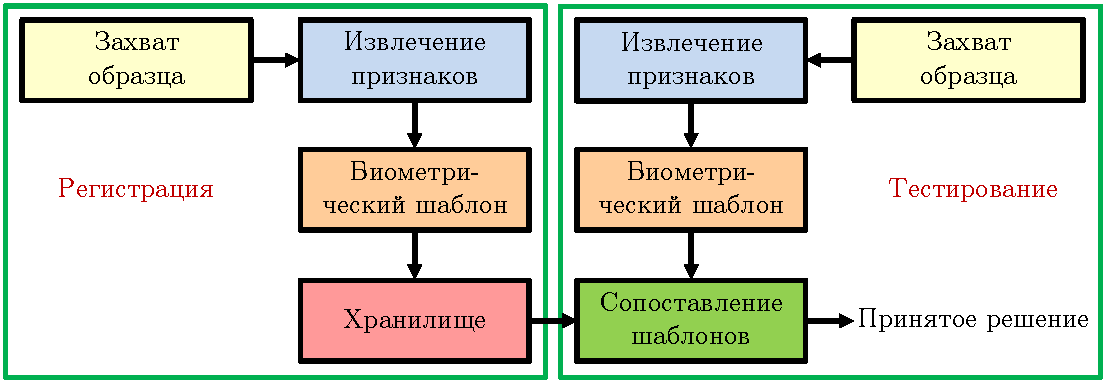
\includegraphics[width=1\linewidth]{images/chapter_01/figure_1_1.pdf}}
\caption{Общая блок-схема биометрической системы: регистрация эталона и сравнение теста с эталоном/эталонами}
\label{fig:figure_1_1}
\end{figure}

К основным \textit{компонентам биометрической системы} можно отнести следующие (см. рис.~\ref{fig:figure_1_1}): 

\begin{itemize}[topsep=1pt] \itemsep0.1em
\item \textit{модуль захвата биометрического образца}, предназначенный для формирования «сырых» данных и их передачи с целью дальнейшей обработки;
\item \textit{модуль извлечения признаков}, выполняющий обработку «сырых» данных с целью извлечения из них характерных, отличительных признаков;
\item \textit{модуль генерации биометрического шаблона}, осуществляющий формирование компактного, высокоуровневого представления биометрического образца;
\item \textit{модуль базы данных/хранилища/галереи}, содержащий биометрические шаблоны, вычисленные для эталонных биометрических образцов, сформированных на этапе регистрации пользователя в системе;
\item \textit{модуль сравнения}, позволяющий выполнить сопоставление биометрического шаблона, выделенного для тестового биометрического образца с шаблоном/шаблонами, содержащимися в базе данных, с целью формирования оценки сравнения, на основе которой принимается биометрическое решение.
\end{itemize}

Рис.~\ref{fig:figure_1_1} показывает, что при использовании биометрической системы первоначально происходит регистрация пользователя в системе. Регистрация сопровождается захватом «сырых» данных, извлечением из них характерных признаков, на основе которых может быть сгенерирован эталонный биометрический шаблон, представленный, обычно, в современных практических приложениях в виде высокоуровневого вектора признаков низкой размерности. Указанный вектор сохраняется в хранилище данных, после чего пользователь считается зарегистрированным в системе. Далее на этапе тестирования выполняется процедура захвата тестового образца, для которого вычисляются признаки и биометрический шаблон. Вычисление признаков и биометрического шаблона на этапе тестирования алгоритмически выполняется идентичным образом, что и на этапе регистрации. Полученный тестовый биометрический шаблон сравнивается с~одним или несколькими эталонами, извлечёнными из хранилища. Результатом сопоставления шаблонов является оценка сравнения, на основе которой принимается биометрическое решение.

Рассматривая биометрические системы в целом, можно выделить следующие основные режимы их работы:

\begin{itemize}[topsep=1pt] \itemsep0.1em
\item \textit{верификация} -- режим, при котором пользователь биометрической системы выдаёт себя за определенную личность. Установление идентичности в данном случае выполняется с помощью оценки схожести между эталонным шаблоном заявленной личности, находящимся в хранилище данных, и предоставленным системе тестовым шаблоном, сформированным в момент взаимодействия пользователя с биометрической системой. Поскольку в результате верификации один эталонный шаблон сопоставляется с одним тестовым шаблоном, подобный режим сравнения определяют как «один к одному». Выходом при этом является ответ «да» или «нет» об аутентичности сравниваемых биометрических шаблонов;

\item \textit{идентификация} -- режим, при котором требуется отнести пользователя биометрической системы к одной из зарегистрированных личностей. При взаимодействии с биометрической системой пользователь не заявляет своё отношение к определённой личности. Поэтому биометрической системе требуется выполнить сравнение предоставленного пользователем тестового биометрического шаблона со всеми эталонными шаблонами зарегистрированных личностей. Подобный режим работы биометрической системы рассматривают в качестве сравнения «один ко многим», а выходом является метка личности, к которой отнесён пользователь биометрической системы.
\end{itemize}

\textit{Производительность и точность работы биометрической системы} зависят от данных, которые подвержены воздействию условий окружающей среды и ограничениям, связанным с технической реализацией системы. В~качестве факторов окружающей среды, воздействующих на биометрическую систему, можно выделить температуру, влажность, освещённость и~т.п. К факторам технической реализации биометрической системы можно отнести следующие: возможность качественного формирования биометрического образца, состав группы пользователей биометрической системы, временной интервал между формированием эталонного и тестового шаблонов, робастность используемых при построении биометрической системы алгоритмов и т.п. Точность работы биометрической системы обычно описывается в терминах ошибок, связанных с формированием биометрического образца и реализационными ограничениями самой системы:

\begin{itemize}[topsep=1pt] \itemsep0.1em
\item \textit{ошибки при формировании биометрического образца} связывают с условиями окружающей среды, в которых эксплуатируется биометрическая система, и качеством сенсора, используемого для захвата биометрического образца. В~качестве примеров подобного рода ошибок можно выделить, во-первых, процент отклонения биометрической системой захваченного образца, из-за его низкого качества и, во-вторых, неспособность сенсора сформировать валидный образец;

\item \textit{ошибки реализационных ограничений системы} используются для оценки точности работы биометрической системы в «полевых» условиях. В~качестве примеров подобного рода ошибок можно выделить \textit{долю ложных отрицательных решений} (англ. false reject rate, FRR, или false negative rate, FNR), также называемую \textit{вероятностью ошибки первого рода}, \textit{долю ложных  положительных решений} (англ. false acceptance rate, FAR или false positive rate, FPR), также называемую \textit{вероятностью ошибки второго рода} и \textit{равный уровень ошибок} (англ. equal error rate, EER). \textit{Доля ложных отрицательных решений} описывает долю событий (в~процентах), когда зарегистрированный в системе пользователь отклонён системой на этапе тестирования. С точки зрения удобства взаимодействия пользователя с системой доля ложных отрицательных решений должна быть меньше настолько, насколько возможно. \textit{Доля ложных положительных решений} описывает долю событий (в~процентах), когда незарегистрированный в системе пользователь не отклонён системой на этапе тестирования. Для робастных биометрических систем доля ложных положительных решений должна быть меньше настолько, насколько возможно. Термин \textit{равного уровня ошибок} относят к такой рабочей точке биометрической системы, для которой доля ложных отрицательных решений и доля ложных положительных решений равны между собой.

\end{itemize}

Вероятно, можно считать, что значимость ошибок, возникающих при формировании биометрического образца, является более важной, чем ошибок, связанных с реализационными ограничениями системы, потому что отсутствие возможности формирования качественных данных, используемых для принятия биометрического решения, драматически влияет на ухудшение качества работы биометрической системы в целом. Например, зачастую гораздо проще повысить качество работы биометрической системы через использование более совершенного сенсора для формирования биометрического образца, чем усложнять алгоритмически конвейер обработки некачественно захваченных данных.
}

\section{Биометрические признаки}

\large{\textit{Биометрические признаки} -- это чёткие, индивидуальные, биологически обусловленные характеристики каждого человека. Применительно к критериям, представленным в пункте~\ref{sec:section_1_1}, можно ввести следующую классификацию биометрических признаков \cite{unar_2014}:

\begin{itemize}[topsep=1pt] \itemsep0.1em
\item \textit{физиологические признаки} -- атрибуты, относящиеся к физиологии человека. Для удобства физиологические признаки могут быть разделены на подкатегории, соответствующие области расположения атрибутов на теле человека (область руки, область лица, область глаза). Дополнительно к физиологическим признакам можно отнести медико-химические атрибуты;
\item \textit{поведенческие признаки} -- атрибуты, относящиеся к особенностям поведения человека;
\item \textit{«мягкие» признаки} -- атрибуты, которые не могут быть использованы самостоятельно при распознавании личности, т.к. определяют её неоднозначно, и, обычно, выступают в качестве дополнительных признаков к~физиологическим и поведенческим.
\end{itemize}

\begin{table}[h]
\centering
\caption{\label{tab:table_1_2}Классификация биометрических признаков}

\begin{tabular}{|cll|}
\hline
\multicolumn{3}{|c|}{Биометрические признаки}                                                                          \\ \hline
\multicolumn{1}{|c|}{Физиологические} & \multicolumn{1}{c|}{Поведенческие} & \multicolumn{1}{c|}{«Мягкие»}             \\ \hline
\multicolumn{1}{|l|}{\begin{tabular}[c]{@{}l@{}}\textit{Область руки:} отпечаток пальца, \\ отпечаток ладони, геометрия руки, \\ вены на руке, отпечаток сгиба пальца\\ \textit{Область лица:} изображение лица, \\ форма уха, отпечаток языка, зубы\\ \textit{Область глаза:} радужная оболочка, \\ сетчатка, сосудистая сеть склеры \\ \textit{Медико-химические признаки:} запах \\ тела, ДНК, электрокардиограмма, \\ звук сердца \end{tabular}} & \multicolumn{1}{l|}{\begin{tabular}[c]{@{}l@{}}Голос, ритм печати \\ текста на клавиатуре, \\ подпись, походка\end{tabular}} & \begin{tabular}[c]{@{}l@{}}Пол, этничность, \\ рост, шрамы, \\ родинки, \\ татуировки\end{tabular} \\ \hline
\end{tabular}
\end{table}

Более подробная детализация того, что собой представляют физиологические, поведенческие и «мягкие» признаки, представлена в табл.~\ref{tab:table_1_2}.}

\subsection{Физиологические признаки в области руки}

\large{Рука человека содержит богатую текстурную информацию, извлечение которой являлось основой для работы ранних систем распознавания личности на основе отпечатков пальцев. В дополнение к отпечаткам пальцев в качестве атрибутов личности в области руки можно выделить отпечаток ладони, геометрию руки, рисунок вен на руке и отпечаток сгиба пальца (см. рис.~\ref{fig:figure_1_2}). Необходимо отметить, что по своей сути подходы распознавания личности на основе различных атрибутов в области руки являются расширением технологии распознавания отпечатков пальцев \cite{unar_2014, minaee_2023}.}

\begin{figure}[h]
\center{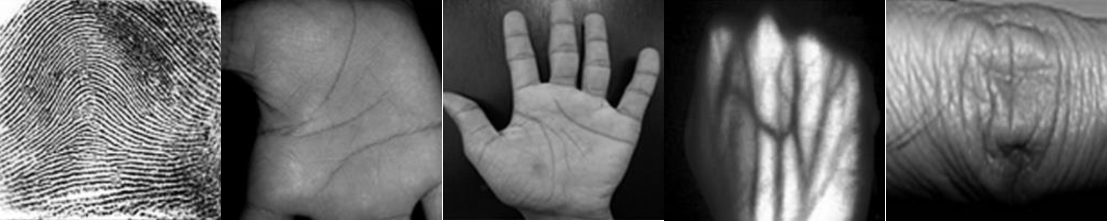
\includegraphics[width=1\linewidth]{images/chapter_01/figure_1_2.pdf}}
\caption{Биометрические признаки в области руки (слева направо): отпечаток пальца, отпечаток ладони, геометрия руки, рисунок вен на руке, отпечаток сгиба пальца. Изображения, представленные на рисунке, позаимствованы из источника \cite{unar_2014}}
\label{fig:figure_1_2}
\end{figure}

\large{\textit{Отпечатки пальцев} (англ. fingerprint) формируются рельефными папиллярными гребнями, которые проходят по поверхности кожи. У людей, как и у некоторых млекопитающих, папиллярные гребни присутствуют на пальцах рук и ладонях, пальцах и ступнях ног. Эволюция формы гребней способствовала улучшению сцепления с поверхностью и передвижения. Потоки папиллярных гребней часто формируют шаблоны, а сами гребни не всегда идут непрерывно, из-за разрывов и отклонений в их структуре. Места, где гребни заканчиваются и разветвляются называются \textit{минуциями} (англ. minutiae). Возникновение минуций носит случайный характер и может быть использовано для распознавания личности, поскольку ни на одном участке кожи, содержащем систему папиллярных гребней, не существует одинаково расположенных минуций. Следовательно, отпечатки пальцев на каждом пальце человека уникальны и могут быть использованы для распознавания личности. Аналогичное можно отметить и по отношению к \textit{отпечатку ладони} (англ. palmprint), при этом площадь рельефной поверхности кожи намного больше и, следовательно, содержит больше деталей для распознавания личности \cite{unar_2014, minaee_2023, gao_2025}. Биометрические системы захватывают и оцифровывают характерные особенности отпечатков пальцев, расположение минуций, поток и ориентацию гребней, для создания биометрического шаблона. Сохранённые в специальное хранилище шаблоны могут быть использованы в дальнейшем для решения задачи распознавания личности. Формирование отпечатков пальцев может быть выполнено с помощью бумаги и чернил, но большинство современных биометрических систем используют специальный сканер, где палец размещается на определённой поверхности или прокатывается по ней. Так же может быть использован бесконтактный метод фиксации, который позволяет захватить требуемую деталь на близком расстоянии. Последний подход является удобным с точки зрения решения проблемы гигиены, связанной с множественными физическими контактами пользователей с поверхностью датчика.} 

\large{Биометрические системы, работающие с \textit{геометрией руки} (англ. hand geometry), используют геометрию пальцев, поверхность руки и её боковой профиль для построения биометрического шаблона \cite{unar_2014, taher_2022}. Изображение геометрии руки выполняется, когда она располагается ладонью вниз на опорной пластине и удерживается в фиксированном положении, например, с помощью направляющих цилиндрических стержней \cite{taher_2022}. Длина, ширина, толщина и площадь поверхности руки распознаваемой личности измеряются и регистрируются. В процессе работы биометрической системы может быть сформировано несколько изображений одной и той же руки, чтобы создать единый шаблон, который содержит достаточно деталей для распознавания личности. На этапе регистрации полученный шаблон помещается в хранилище и используется в будущих взаимодействиях пользователя с системой, когда рука субъекта снова размещается на опорной пластине в определённом положении, чтобы получить биометрический шаблон, который сравнивается с шаблоном, помещённым в хранилище.}

\large{Биометрические системы, основанные на использовании \textit{рисунка вен на руке} (англ. hand vein pattern), анализируют разветвления и окончания вен под кожей человеческой руки \cite{unar_2014, tamimi_2019, hemis_2024}, а использование \textit{отпечатка сгиба пальца} (англ. finger knuckle print) для распознавания личности предполагает фиксацию текстуры линий на внешней части пальца в области фалангового сустава \cite{unar_2014, tarawneh_2022}. Всё же нужно отметить, что технология распознавания личности по отпечаткам пальцев занимает доминирующую позицию среди систем, использующих биометрические признаки в области руки. Последнее связано с тем, что данная технология существует достаточно давно, обладает более высокой степенью уникальности, а также высокой приемлемостью при использовании, что делает её подходящей для распознавания личности. Низкая стоимость датчиков и малый размер биометрического шаблона делают использование атрибутов личности в области руки привлекательными для практических приложений. В то же время физический контакт с устройством формирования изображения, заболевания рук, шрамы, порезы, влажная и сухая кожа, а также загрязнённая и маслянистая поверхность датчиков являются некоторыми проблемами, связанными с использованием данной биометрической технологии.}

\subsection{Физиологические признаки в области лица}

\large{Область лица человека представляет собой одну из интересных тем для научных исследований, поскольку лицо является наиболее естественной биометрической особенностью, используемой для распознавания людей на протяжении многих столетий, а признаки в области лица могут быть захвачены бесконтактным способом. В качестве основных биометрических признаков в области лица можно выделить изображение лица в видимой области спектра, термограмму лица, форму уха, а также отпечаток языка (см. рис.~\ref{fig:figure_1_3}).}

\begin{figure}[h]
\center{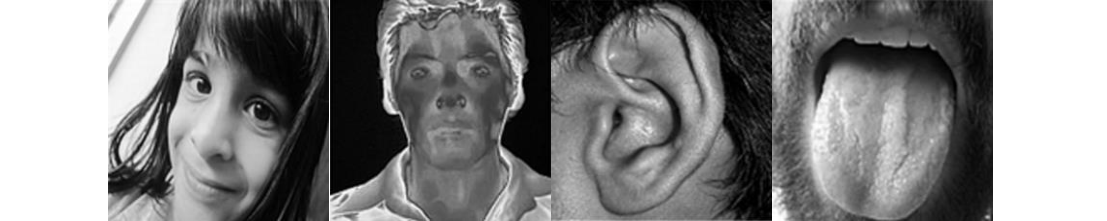
\includegraphics[width=1\linewidth]{images/chapter_01/figure_1_3.pdf}}
\caption{Биометрические признаки в области лица (слева направо): изображение лица в видимой области спектра, термограмма лица, форма уха, отпечаток языка. Изображения, представленные на рисунке, позаимствованы из источника \cite{unar_2014}}
\label{fig:figure_1_3}
\end{figure}

\large{\textit{Распознавание личности по изображению лица в видимой части спектра} (англ. face recognition) является одной из наиболее часто используемых биометрических систем, основанных на применении признаков в области лица \cite{unar_2014, minaee_2023, wang_2022}. Изображение лица может быть захвачено обычной камерой или камерой смартфона в режиме портрета или в процессе записи видео движущегося объекта. Захват изображения может происходить на расстоянии без сотрудничества с объектом съёмки или каких-либо знаний о нём. На данный момент существует множество подходов к статистическому анализу характеристик лица, учитывающих влияние возраста, выражения лица, освещения и других факторов. Подобные подходы могут включать использование алгоритмов машинного обучения, например, нейросетевых, что не подразумевает непосредственного измерения расстояний между основными частями лица. Современные алгоритмы распознавания лиц описывают форму и внешние черты лица (глаза, нос и рот) путём применения алгоритмов обработки изображений, специально обученных на вычисление дискриминативных и стабильных числовых представлений, называемых \textit{лицевыми биометрическими шаблонами}. Необходимо отметить, что схожие подходы могут быть использованы для вычисления основных характеристик лица таких, как возраст, пол, этническое происхождение личности и т.п. Последнее не обязательно подразумевает решение задачи распознавания личности и может использоваться в рамках приложений, связанных с необходимостью разделения людей на отдельные группы. Важно отметить, что системы распознавания лиц не гарантируют надёжного распознавания личности при нанесении косметики или после вмешательства пластической хирургии. Лицо человека изменяется с течением времени, что оказывает влияние на точность работы биометрической системы. В дополнение к указанному, оборудование для захвата и обработки изображений является достаточно дорогостоящим, что может быть ограничивающим фактором при использовании систем распознавания лиц.}

\large{Возможным вариантом для построения более надёжных систем распознавания лиц может являться использование \textit{термограмм лица} (англ. facial thermogram), которые содержат шаблон теплового излучения, исходящего от лица, из-за наличия сосудистой структуры под кожей лица человека \cite{unar_2014, lin_2021}.}

\large{\textit{Форма уха} (англ. ear shape) человека (размер, длина, ширина и высота завитка, треугольной ямки, противозавитка, раковины и т.п.) раскрывает специфические характеристики, которые позволяют выполнить распознавание личности \cite{unar_2014, minaee_2023}. Распознавание личности по форме уха использовалось в течение многих лет в различных странах применительно к задаче идентификации преступников, где данные об ушах подозреваемого собирались совместно с изображением его лица и отпечатками пальцев. С появлениям передовых вычислительных алгоритмов на основе нейронных сетей распознавание личности по форме уха стало жизнеспособной автоматизированной биометрической технологией, выходящей за рамки её традиционных приложений для правоохранительных органов.}

\large{Язык человека является жизненно важным органом, который выполняет множество действий, таких как артикуляция речи, восприятие вкуса и формирование пищевого комка. Использование \textit{отпечатка языка} (англ. tongue print) является одним из возможных вариантов распознавания личности \cite{unar_2014, bhattacharyya_2023}. Потенциальными преимуществами, связанными с отпечатком языка, являются его изолированность и защищённость от внешней среды, а также его подвижность, которая подтверждает витальность (англ. liveness) личности. Cистема распознавания личности по отпечатку языка может использовать геометрические характеристики, такие как ширина, толщина и кривизна контура языка, а также особенности его трещин и текстуры.}

\subsection{Физиологические признаки в области глаза}

\large{Общаясь лично, люди часто смотрят друг другу в глаза, чтобы уловить истинные чувства собеседника. Однако, исследования учёных в значительной степени показали, что можно извлечь гораздо большее, анализируя глаза человека. Распознавание личности с использованием атрибутов в области глаза вошло в биометрические сценарии относительно недавно\footnote{Джон Догман разработал и в 90-х гг. 20-го века запатентовал первый настоящий алгоритм распознавания радужной оболочки глаза человека, опубликовав первые публикации и проведя первые живые демонстрации. Предложенный алгоритм использовал двумерное вейвлет-преобразование Габора для извлечения фазовой структуры радужной оболочки.}, по сравнению, например, с распознаванием на основе отпечатков пальцев или изображения лица человека, обладая более точными, высоконадёжными, стабильными и хорошо защищёнными биометрическими признаками. К основным биометрическим атрибутам в области глаза можно отнести радужную оболочку, сетчатку и сосудистую сеть склеры (см. рис.~\ref{fig:figure_1_4}).}

\begin{figure}[h]
\center{
\includegraphics[width=1\linewidth]{images/chapter_01/figure_1_4.pdf}}
\caption{Биометрические признаки в области глаза (слева направо): радужная оболочка, сетчатка, сосудистая сеть склеры. Изображения, представленные на рисунке, позаимствованы из источника \cite{unar_2014}}
\label{fig:figure_1_4}
\end{figure}

\large{Системы \textit{распознавания личности по радужной оболочке} (англ. iris re- cognition) глаза используют уникальную и стабильную текстуру, состоящую из крипт, борозд, короны и веснушек радужной оболочки глаза человека \cite{unar_2014, minaee_2023, nguyen_2024}. \textit{Радужная оболочка} (англ. iris) выглядит как цветной круглый сегмент передней части глаза, в центре которого находится зрачок. Она контролирует размер зрачка, регулируя количество света, попадающего в глаз. Текстура радужной оболочки в процессе распознавания может быть зафиксирована камерой, работающей в ближнем инфракрасном диапазоне длин волн, либо в видимой части спектра. Первые камеры для захвата достаточного количества деталей радужной оболочки располагались близко к глазам, но не соприкасались с ними. Однако, в настоящее время существует возможность размещать камеры на более далёком расстоянии для захвата радужной оболочки людей, находящихся в движении, например, у посадочного выхода в аэропорту.}

\large{\textit{Сетчатка} (англ. retina) представляет собой тонкий слой нервной ткани, расположенный с внутренней стороны задней части глазного дна, обеспечивающий восприятие и преобразование электромагнитного излучения видимой части спектра в нервные импульсы, а также выполняющий их первичную обработку. Кровоснабжение сетчатки осуществляется за счёт сети кровеносных сосудов, которая образует уникальную структуру, позволяющую выполнить распознавание личности путём анализа положения и бифуркаций кровеносных сосудов, а также измерения площади центральной ямки (англ. fovea) и диска зрительного нерва (англ. optic disk) \cite{unar_2014}.}

\large{\textit{Склера} (англ. sclera) является наружной плотной белковой оболочкой глаза, в передней части переходящей в роговицу. При движении глаза влево или вправо становится видна сосудистая сеть (англ. vasculature). Сосудистая сеть склеры может быть использована для распознавания личности \cite{unar_2014, rot_2020, derakhshani_2006}, представляя относительно новый подход, предложенный в первом десятилетии 2000-х гг. Изображения сосудистой сети склеры могут быть получены с помощью обычной камеры, инфракрасной камеры или с использованием камеры смартфона.}

\large{Высокая уникальность, стабильность с течением времени, высокая безопасность и сложность подделки атрибутов в области глаза делают распознавание личности на их основе подходящим для практических приложений. Однако, чувствительность к освещению, более сложное взаимодействие пользователя с системой, высокая стоимость датчиков изображений, а также отражения, возникающие от источников окружающего света, являются некоторыми проблемами при использовании подобных биометрических систем.}

\subsection{Медико-химическая биометрия}

\large{Запах тела, дезоксирибонуклеиновая кислота или ДНК, электрокардиограмма или ЭКГ и звук сердца рассматриваются в качестве \textit{медико-хими- ческих физиологических признаков} \cite{unar_2014}, поскольку процесс распознавания личности в данном случае требует использования специализированных ме- дицинских/химических датчиков. Необходимо отметить, что \textit{ДНК} (англ. deoxyribonucleic acid, DNA) является хорошо известным и наиболее точным биометрическим атрибутом, доминирующим над другими видами медико-химических признаков. Одномерный код ДНК обычно извлекается из не- большой изменяющейся области целого кода, называемой \textit{микросаттелитом} или \textit{коротким тандемным повтором} (англ. short tandem repeat) через получение образцов крови, волос, ушной серы, обрезков ногтей и т.п. \textit{Запах тела} (англ. body odor), представляющий собой композицию различных органических соединений, может быть захвачен с помощью массива химических сенсоров, чувствительных к этим соединениям, с целью дальнейшего биометрического анализа. Некоторые исследования, основанные на анализе \textit{кепстральных коэффициентов звука сердца} (англ. cepstral coefficients of heart sound) и анализе \textit{реперных точек} (англ. fiducial points) из данных \textit{ЭКГ} (англ. electrocardiogram, ECG), демонстрируют многообещающие результаты применительно к задаче распознавания личности. Не- обходимо отметить, что инвазивная процедура сбора данных, проблемы конфиденциальности, физический контакт с датчиками, необходимость наличия опытных операторов, полное сотрудничество со стороны субъектов и зависимость от медицинского и эмоционального состояния человека являются некоторыми из ограничений для крупномасштабного развёртывания биометрических систем, основанных на использовании медико-химических признаков.}

\subsection{Поведенческая биометрия}

\large{\textit{Поведенческие атрибуты} \cite{unar_2014} позволяют выполнить распознавание личности на основе того, как люди выполняют определённые вещи. Характеристики голоса человека, стиль набора текста на клавиатуре (динамика нажатия клавиш), динамика подписи и походка человека являются примерами поведенческих атрибутов (см. рис.~\ref{fig:figure_1_5}).}

\begin{figure}[]
\center{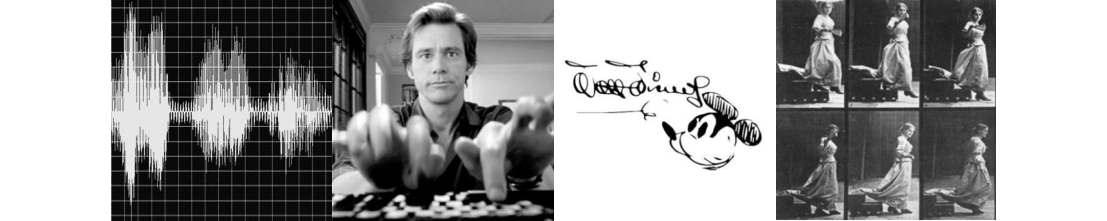
\includegraphics[width=1\linewidth]{images/chapter_01/figure_1_5.pdf}}
\caption{Поведенческая биометрия (слева направо): осциллограмма речевого сигнала, ритм печати текста на клавиатуре (кадр из фильма «Брюс всемогущий»), подпись Уолта Диснея, походка на примере фотографий Эдварда Майбриджа «Женщина, спускающаяся по лестнице». Изображения позаимствованы из общедоступных интернет-источников}
\label{fig:figure_1_5}
\end{figure}

\large{\textit{Голос} (англ. voice) человека состоит из звуков, формируемых с помощью голосового тракта в процессе разговора, пения, смеха, плача, крика и т.п. Система \textit{распознавания диктора} \cite{unar_2014, minaee_2023, hansen_2015, bai_2021} использует его голосовые характеристики (частотный cпектр, частота основного тона, ритм, акцент, произношение и т.п.) для установления личности либо с учётом ограничений на некоторую заранее определённую фразу, \textit{текстозависимое распознавание}, которую требуется произнести, либо без них, \textit{текстонезависимое распознавание}. Голос человека может быть захвачен с помощью микрофона, оцифрован и проанализирован специально обученными моделями, позволяющими сформировать \textit{голосовой биометрический шаблон}, необходимый для распознавания личности. 

\textit{Распознавание личности по стилю набора текста на клавиатуре} (англ. keystroke dynamics recognition) \cite{unar_2014, sharma_2023} основано на анализе времени выбора, нажатия и отпускания определённых клавиш, базовой динамики и ритма нажатия клавиш, ловкости каждой руки и распространённых повторяющихся ошибок.

Использование рукописных подписей для аутентификации бумажных документов имеет долгую историю. В настоящее время применение современных электронных биометрических методов автоматизировало этот процесс. Системы \textit{распознавания личности на основе подписи} (англ. signature recognition) \cite{unar_2014, minaee_2023} выполняют анализ характеристик подписи человека, представленной системе, либо в статическом, либо в динамическом режиме. \textit{Статическое распознавание подписи} предполагает предварительное формирование цифрового эталонного шаблона на основе графического изображения рукописной подписи. Последующие подписи предоставляются в ходе деловой деятельности, например, на чеках, контрактах и т.п., а характеристики подписей, форма, размер, изгибы и т.п., сравниваются алгоритмически с эталонной подписью. \textit{Динамическое распознавание подписи} предполагает электронную фиксацию физических действий, связанных с написанием подписи. Как правило, это выполняется с использованием устройства, обладающего сенсорным экранов, например, планшета. Поэтому в качестве основных характеристик для распознавания личности в данном случае могут использоваться трехмерная оценка затраченного времени, ритм и различные скорости формирования каждой буквы и всей подписи, величина давления пера/стилуса и направления штрихов.

У каждого человека есть своя собственная манера ходьбы и бега. Такие характеристики, как общее телосложение субъекта, длина и ширина шага, скорость движения, различные углы, образуемые суставами бедра, колена и лодыжки, а также углы туловища, бёдер и стоп, могут быть зафиксированы камерой для дальнейшего анализа. Анализ  указанных характеристик позволяет выполнить \textit{распознавание личности по стилю походки} (англ. gait recognition) \cite{unar_2014, minaee_2023, shen_2022}, а также может быть использован при проведении медицинских исследований и диагностического тестирования, в спортивной науке и т.п.

Детальный анализ поведенческих атрибутов показывает, что они подвержены влиянию эмоционального состояния человека, состояния здоровья, пищевых привычек и старения организма, ухудшающих качество работы биометрической системы. Однако, низкая вычислительная стоимость при приемлемом качестве может являться плюсом систем поведенческой биометрии.

}

\subsection{«Мягкая» биометрия}

\large{Начало развития «мягкой» биометрия \cite{unar_2014} было положено во второй половине 19-го века Альфонсом Бертильоном, который разработал систему идентификации преступников по их антропометрическим данным. \textit{Основной особенностью атрибутов «мягкой» биометрии} является то, что они не обладают отличительными и постоянными свойствами, и являются часто встречающимися среди различных людей. Поэтому данные атрибуты используются, как правило, в качестве дополнения к физиологическим и поведенческим признакам при распознавании личности, будучи вычисленными за минимально возможное время. В качестве примера «мягких» биометрических атрибутов можно привести этничность, рост и вес, пол, цвет кожи, глаз и волос, а также шрамы, родинки и татуировки (см. рис.~\ref{fig:figure_1_6}).}

\begin{figure}[]
\center{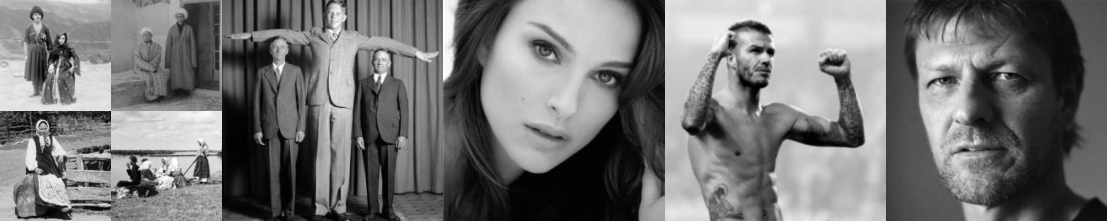
\includegraphics[width=1\linewidth]{images/chapter_01/figure_1_6.pdf}}
\caption{Примерами признаков, используемых в «мягкой» биометрии, являются этничность (фотографии народов Российской империи, сделанные Сергеем Михайловичем Прокудиным-Горским), рост (фотография Роберта Уодлоу), родинки (фотография Натали Портман), татуировки (фотография Дэвида Бекхема), шрамы (фотография Шона Бина). Изображения позаимствованы из общедоступных интернет-источников}
\label{fig:figure_1_6}
\end{figure}

\large{Поскольку «мягкие» биометрические атрибуты не обладают достаточной дискриминативностью для распознавания личности, они могут использоваться в процессе категоризации данных, что в конечном итоге уменьшает время распознавания, а также увеличивает точность, сужая пространство поиска.}

\section{Мультимодальная биометрия}

\large{Здесь какой-то текст!}

\section{Голосовая биометрическая система}

\large{Здесь какой-то текст!}

\section{Основные задачи, решаемые голосовой биометрической~системой}

\large{Здесь какой-то текст!}

\section{Конвейер голосовой биометрии}

\large{Здесь какой-то текст!}

\section{Критерии надёжности систем голосовой биометрии}

\large{Здесь какой-то текст!}

\section{Примеры практического использования систем голосовой~биометрии}

\large{Здесь какой-то текст!}

\section{Биометрические стандарты}

\large{Здесь какой-то текст!}

\section{Почему распознавание диктора -- сложная задача?}

\large{Здесь какой-то текст!}

\section{Текущее состояние дел в области голосовой биометрии}

\large{Здесь какой-то текст!}

\section{Нерешённые проблемы и перспективные направления в~области голосовой биометрии}

\large{Здесь какой-то текст!

\section*{Контрольные вопросы}

\large{

\begin{enumerate}
\item Что такое биометрия?
\item В чём состоят основные преимущества биометрии перед знанием пароля и использованием карты?
\item Каким основным критериям должны удовлетворять биометрические признаки?
\item Как можно классифицировать биометрические признаки?
\item Что такое биометрическая система?
\item Из каких основных модулей состоит биометрическая система?
\end{enumerate}

}

\renewcommand{\bibname}{Список литературы}

\vspace{0mm}

\begin{thebibliography}{11}
    \thispagestyle{fancy}
    \addcontentsline{toc}{section}{\bibname}
    
    \bibitem{unar_2014} Unar J.A., Seng W.C., Abbasi A. A review of biometric technology along with trends and prospects // Pattern Recognition. -- 2014. -- V. 47. -- No.~8. -- P. 2673-2688.

    \bibitem{kukharev_2013} Методы обработки и распознавания изображений лиц в задачах биометрии / Г.А. Кухарев [и др.] -- СПб: Политехника, 2013. -- 388 с.

    \bibitem{tripathi_2011} Tripathi K.P. A comparative study of biometric technologies with reference to human interface // Int. J. Computer Applications. -- 2011. -- V. 14. -- No. 5. -- P. 10-15.

    \bibitem{dahea_2018} Dahea W., Fadewar H.S. Multimodal biometric system: a review // Int. J. Research in Advanced Engineering and Technology. -- 2018. -- V. 4. -- No.~1. -- P. 25-31.

    \bibitem{rousan_2020} Al-Rousan M., Intrigila В. A comparative analysis of biometrics types: literature review // J. Computer Science. -- 2020. -- V. 16. -- No. 12. -- P.~1778-1788. 

    \bibitem{minaee_2023} Minaee S. et al. Biometrics recognition using deep learning: a survey // Artificial Intelligence Review. -- 2023. -- V. 56. -- No. 8. -- P. 8647-8695.

    \bibitem{gao_2025} Gao C. et al. Deep learning in palmprint recognition -- a comprehensive survey // arXiv preprint arXiv:2501.01166. -- 2025.

    \bibitem{taher_2022} Taher M.M., George L.E. A digital signature system based on hand geometry -- survey // Wasit J. Computer and Mathematic Science. -- 2022. -- V. 1. -- No. 1. -- P. 1-14.

    \bibitem{tamimi_2019} Al-Tamimi M.S.H. A survey on the vein biometric recognition systems: trends and challenges // J. Theoretical and Applied Information Technology. -- 2019. -- V. 97. -- No. 2. -- P. 551-568.

    \bibitem{hemis_2024} Hemis M. et al. Deep learning techniques for hand vein biometrics: a comprehensive review // Information Fusion. -- 2024. -- P. 102716.

    \bibitem{tarawneh_2022} Tarawneh A.S. et al. DeepKnuckle: deep learning for finger knuckle print recognition // Electronics. -- 2022. -- V. 11. -- No. 4. -- P. 513.

    \bibitem{wang_2022} Wang X. et al. A survey of face recognition // arXiv preprint arXiv:2212.13038. -- 2022.

    \bibitem{lin_2021} Lin S.D., Chen L., Chen W. Thermal face recognition under different conditions // BMC Bioinformatics. -- 2021. -- V. 22. -- P. 1-17.

    \bibitem{bhattacharyya_2023} Bhattacharyya A. et al. Tongue print: a unique biometric and potential forensic tool: a Review // Oral and Maxillofacial Pathology J. -- 2023. -- V. 14. -- No. 2. P. 208-210.

    \bibitem{nguyen_2024} Nguyen K., Proença H., Alonso-Fernandez F. Deep learning for iris recognition: a survey // ACM Computing Surveys. -- 2024. -- V. 56. -- No. 9. -- P. 1-35.

    \bibitem{rot_2020} Rot P. et al. Deep sclera segmentation and recognition // Handbook of Vascular Biometrics. -- 2020. -- P. 395-432.

    \bibitem{derakhshani_2006} Derakhshani R., Ross A., Crihalmeanu S. A new biometric modality based on conjunctival vasculature // Proc. Artificial Neural Networks in Engineering (ANNIE). -- 2006. -- P. 1-8.

    \bibitem{hansen_2015} Hansen J.H.L., Hasan T. Speaker recognition by machines and humans: a tutorial review // IEEE Signal Processing Magazine. -- 2015. -- V. 32. -- V.~6. -- P. 74-99.
    
    \bibitem{bai_2021} Bai Z., Zhang X.L. Speaker recognition based on deep learning: an overview~// Neural Networks. -- 2021. -- V.~140. -- P.~65-99.

    \bibitem{sharma_2023} Sharma A., Jureček M., Stamp M. Keystroke dynamics for user identification // arXiv preprint arXiv:2307.05529. --- 2023.

    \bibitem{shen_2022} Shen C. et al. A comprehensive survey on deep gait recognition: algorithms, datasets and challenges // arXiv preprint arXiv:2206.13732. -- 2022.

\end{thebibliography}

\end{document}
